\documentclass{article}
\usepackage[margin=1in]{geometry}
\usepackage{amsmath,amsthm,amssymb}
\usepackage{bbm,enumerate,mathtools}
\usepackage{tikz,pgfplots}
\usepackage{chessboard}
\usepackage[hidelinks]{hyperref}
\usepackage{multicol} % Problem 35
\usepackage{xstring} % Difficulty command
\usetikzlibrary{shapes.geometric}

\newenvironment{question}{\begin{trivlist}\item[\textbf{Question.}]}{\end{trivlist}}
\newenvironment{note}{\begin{trivlist}\item[\textbf{Note.}]}{\end{trivlist}}
\newenvironment{references}{\begin{trivlist}\item[\textbf{References.}]}{\end{trivlist}}
\newenvironment{related}{\begin{trivlist}\item[\textbf{Related.}]\end{trivlist}\begin{enumerate}}{\end{enumerate}}

\newcommand\score[1]{
\pgfmathsetmacro\pgfxa{#1+1}
\tikzstyle{scorestars}=[
  star,
  star points=5,
  star point ratio=2.25,
  draw,
  inner sep=3pt,
  anchor=outer point 5
]
  \begin{tikzpicture}[baseline]
    \draw[opacity=0] (0,-0.5) rectangle (0,0.2); % Workaround for whitespace at the bottom.
    \foreach \i in {1,...,4} {
      \pgfmathparse{(\i<=#1?"yellow":"gray")}
      \edef\starcolor{\pgfmathresult}
      \draw (\i*4.5ex,0) node[name=star\i,scorestars,fill=\starcolor]  {};
    }
  \end{tikzpicture}
}

\newcommand{\difficulty}[1]{%
  \IfEqCase{#1}{%
      {1}{
        
\begin{tikzpicture}[scale=0.7, baseline=0.9mm]%
          \definecolor{slopegreen}{rgb}{0.0, 0.5, 0.0}%
          \fill[slopegreen] (0.5,0.5) circle (0.5);%
        \end{tikzpicture}%
      }%
      {2}{
        
\begin{tikzpicture}[scale=0.7, baseline=0.9mm]%
          \definecolor{slopeblue}{rgb}{0.0, 0.44, 1.00}
          \fill[slopeblue] (0,0) rectangle (1,1);%
        \end{tikzpicture}%
      }%
      {3}{
\begin{tikzpicture}[scale=0.7, baseline=0.9mm]\fill (0,0.5)--(0.5, 0)--(1,0.5)--(0.5,1)--cycle; \end{tikzpicture}}%
      {4}{
\begin{tikzpicture}[scale=0.7, baseline=0.9mm]\fill (0.25,0)--(0,0.5)--(0.25,1)--(0.5,0.5)--cycle; \fill (0.75,0)--(0.5,0.5)--(0.75,1)--(1,0.5)--cycle;\end{tikzpicture}}%
      % you can add more cases here as desired
  }[\PackageError{difficulty}{Undefined difficulty level: #1}{}]%
}%
\newcommand{\rating}[2]{\difficulty{#1}\\\score{#2}\\}


\begin{document}
\rating{3}{4}
Consider the fuction A300002(n) which is the lexicographically earliest
sequence of positive integers such that no $k + 2$ points are on a polynomial
of degree $k$. (i.e. no two points are equal, no three points are colinear, no
four points are on a parabola, etc.)
\begin{figure}[!h]
  \centering
  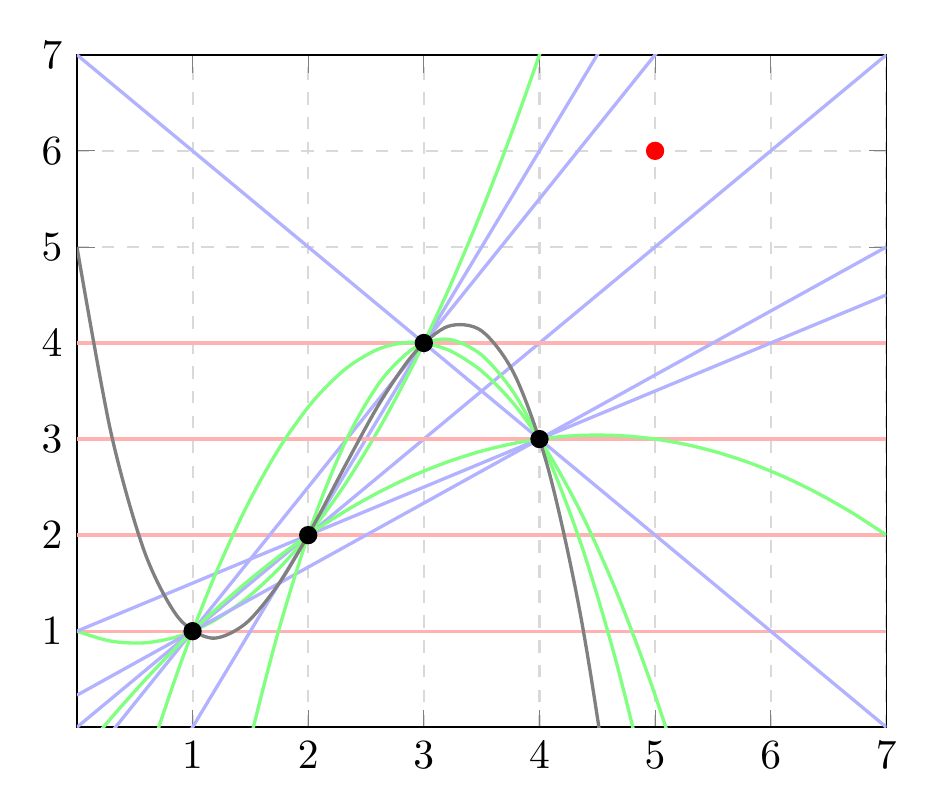
\begin{tikzpicture}[scale=1.5]
    \begin{axis}[
      xmin=0, xmax=7,
      ymin=0, ymax=7,
      domain=0:7,
      grid=both,
      grid style={line width=0.5pt, draw=gray!30, dashed},
      ytick={1,...,7},
      xtick={1,...,7},
      smooth
    ]
      \addplot[red!30, thick] (x,1);

      \addplot[red!30, thick] (x,2);
      \addplot[blue!30, thick] (x,x);

      \addplot[red!30, thick] (x,4);
      \addplot[blue!30, thick] (x,2*x-2);
      \addplot[blue!30, thick] (x,1.5*x-0.5);
      \addplot[green!50, thick] (x,{(x^2 - x)/2 + 1});

      \addplot[red!30, thick] (x,3);
      \addplot[blue!30, thick] (x,{(2/3)*x + (1/3)});
      \addplot[blue!30, thick] (x,0.5*x + 1);
      \addplot[blue!30, thick] (x,-x + 7);
      \addplot[green!50, thick] (x,{-x^2/6 + (3*x)/2 - 1/3});
      \addplot[green!50, thick] (x,{-(5*x^2)/6 + (29*x)/6 - 3});
      \addplot[green!50, thick] (x,{-(3*x^2)/2 + (19*x)/2 - 11});
      \addplot[gray, thick] (x,{-(2*x^3)/3 + (9*x^2)/2 - (47*x)/6 + 5});

      \addplot[mark=*] coordinates {(1,1)};
      \addplot[mark=*] coordinates {(2,2)};
      \addplot[mark=*] coordinates {(3,4)};
      \addplot[mark=*] coordinates {(4,3)};
      \addplot[mark=*, red] coordinates {(5,6)};
    \end{axis}
  \end{tikzpicture}
  \caption{
    The first four points together with all interpolated polynomials.
    The red point marks the lowest integer coordinate $(5, k)$ that does not
    lie on an interpolated polynomial. (Degree 0 polynomials are plotted in red,
    degree 1 in blue, degree 2 in green and degree 3 in gray.)
  }
\end{figure}

\begin{question}
  Do all positive integers occur in this sequence?
\end{question}

\begin{related}
  \item What is the asymptotic growth of this sequence?
  \item Does \textit{any} permutation of the natural numbers have the property
  that no $k + 2$ points are on a polynomial of degree $k$?
\end{related}

\begin{references}
  \item \url{https://oeis.org/A300002}
\end{references}
\end{document}
